\documentclass{article}
\usepackage[utf8]{inputenc}
\usepackage{listings}
\usepackage{xcolor}
\usepackage{subcaption}
\usepackage{minted}

\definecolor{codegreen}{rgb}{0,0.6,0}
\definecolor{codegray}{rgb}{0.5,0.5,0.5}
\definecolor{codepurple}{rgb}{0.58,0,0.82}
\definecolor{backcolour}{rgb}{0.95,0.95,0.92}
\usepackage{color}   %May be necessary if you want to color links
\usepackage{hyperref}
\usepackage{graphicx}
\hypersetup{
    colorlinks=true, %set true if you want colored links
    linktoc=all,     %set to all if you want both sections and subsections linked
    linkcolor=black,  %choose some color if you want links to stand out
    urlcolor=blue,
}
\lstdefinestyle{mystyle}{
    backgroundcolor=\color{backcolour},   
    commentstyle=\color{codegreen},
    keywordstyle=\color{magenta},
    numberstyle=\tiny\color{codegray},
    stringstyle=\color{codepurple},
    basicstyle=\ttfamily\footnotesize,
    breakatwhitespace=false,         
    breaklines=true,                 
    captionpos=b,                    
    keepspaces=true,                 
    numbers=left,                    
    numbersep=5pt,                  
    showspaces=false,                
    showstringspaces=false,
    showtabs=false,                  
    tabsize=2
}

\lstset{style=mystyle}


\title{SMBUD}
\author{Filippo Lazzati, Martina Magliani, Christian Grasso, Sofia Martellozzo, Giacomo Lombardo}
%\date{October 2021}

\begin{document}
\thispagestyle{empty}
\begin{titlepage}
    \begin{center}
       %\vspace*{2cm}
       {\Huge \textbf{SMBUD}} %%Replace this with the Title of your research
       \vspace{0.5cm}
       \\
    \begin{LARGE}
        {Vaccinations Analysis}
        \vspace{1.0cm}
        \\
        {\textit{Specification, Entity-Relationship model and Elasticsearch analysis}}
           
\includegraphics[width=13cm]{polimi.png}
          \vspace{1.5cm}\\
                  Filippo Lazzati (10629918) - Martina Magliani (10682333) - Christian Grasso (10652464) - Sofia Martellozzo (10623060) - Giacomo Lombardo (10674987)\\
       {Year: 2021/2022}
    \end{LARGE}  
   \end{center}
\end{titlepage}
\newpage
\tableofcontents %this command creates an index
\newpage
\section{Problem specification}
The purpose of this project is to design, store and query data on a NoSQL database in order to analyze data about COVID-19 vaccination statistics.\\ Starting from an open dataset containing raw data about the distribution and administering of COVID-19 vaccines in Italian regions, the main goal of the project is to obtain relevant information through queries and graphs.\\
To perform this task, the dataset has been loaded into \textbf{ElasticSearch}, a search engine with an internal database focused on high performances that interacts with external components through RESTful APIs. Once loaded into the search engine, information can be retrieved from the dataset not only through queries but also through Kibana, a powerful user interface that allows to visualize ElasticSearch data. More specifically, through \textbf{Kibana} it is possible to create Dashboards that generate and display graphs and other significant information in an intuitive way.\\
\subsection{Dataset}
The used dataset is provided by the Italian Government and contains the official data about vaccines distribution and administration. More specifically it provides regional overview of the amount of doses administered daily in the time period between 27/12/2020 and today.
The daily administration are divided by:
\begin{itemize}
    \item type of dose (first, second, booster and post-infection)
    \item supplier (Pfizer, Moderna,...)
    \item age group
    \item gender
    \item area
\end{itemize}
A secondary dataset, containing additional information about the amount of daily delivered doses in the same time period, has also been implemented in order to better contextualise the primary dataset. 

\newpage

%---------------------------------%
\section{Conceptual model}
The following is the Entity-Relationship (E-R) model of our database:\\ \\ \\
\vspace{1cm}
%--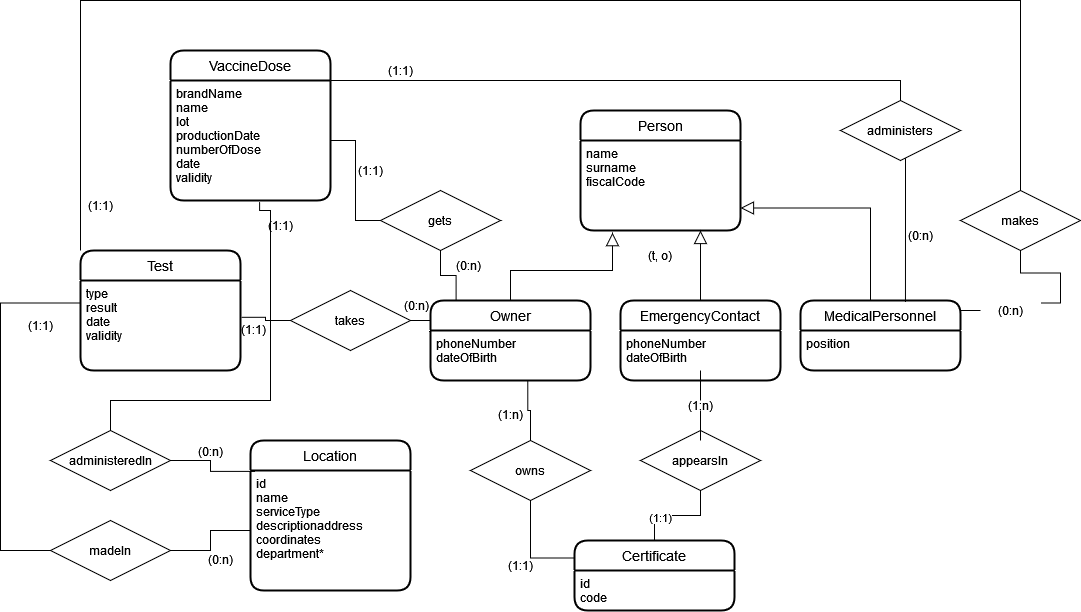
\includegraphics[trim=1cm 1cm 1cm 1cm, width=15cm]{images/e-r.png}
\begin{itemize}
    \item 
\end{itemize}
\newpage

%---------------------------------%
\section{Sample dataset}

\subsection{Import the dataset}\label{import}

\newpage
%---------------------------------%
\section{Queries and Commands}
---

\subsection{Queries}
We have identified the following queries:
\begin{enumerate}
\item \textbf{list of brands with number of vaccinations in last 30 days and brand with the highest number}.\\
\begin{lstlisting}
GET /somministrazioni-vaccini-latest/_search
{
  "size": 0,
  "query": {
    "range": {
      "@timestamp": {
        "gte": "now-30d/d",
        "lt": "now/d"
      }
    }
  },
  "runtime_mappings": {
    "vaccini": {
      "type": "long",
      "script": """
        long total = doc['sesso_maschile'].value + doc['sesso_femminile'].value;
        emit(total);
      """
    }
  },
  "aggs": {
    "vaccinations_per_brand": {
      "terms": {
        "field": "fornitore"
      },
      "aggs": {
        "total_vaccinations": {
          "sum": {
            "field": "vaccini"
          }
        }
      }
    }
  ,
    "most-used_brand": {
      "max_bucket": {
        "buckets_path": "vaccinations_per_brand > total_vaccinations" 
      }
  }
}
}
\end{lstlisting}
\item \textbf{region with highest number of 1st vaccinations in last 3 months}.\\
\begin{lstlisting}
GET /somministrazioni-vaccini-latest/_search
{
  "size": 0,
  "query": {
    "range": {
      "@timestamp": {
        "gte": "now-90d/d",
        "lt": "now/d"
      }
    }
  },
  "aggs": {
    "first_vaccinations_per_region": {
      "terms": {
        "field": "area"
      },
"aggs": {
        "first_vaccinations": {
          "sum": {
            "field": "prima_dose"
          }
        }
}
  },
    "most-vaccinated_region": {
      "max_bucket": {
        "buckets_path": "first_vaccinations_per_region > first_vaccinations" 
      }
  }
}
}

\end{lstlisting}
\item \textbf{total number of boosters in italy in last 30 days}.\\
\begin{lstlisting}
GET /somministrazioni-vaccini-latest/_search
{
  "size": 0,
  "query": {
    "range": {
      "@timestamp": {
        "gte": "now-30d/d",
        "lt": "now/d"
      }
    }
  },
  "aggs": {
    "total_number_of_boosters": {
      "sum": {
        "field": "dose_addizionale_booster"
      }
  }
  }
}
\end{lstlisting}
\item \textbf{age range with highest number of vaccinations in last 30 days}
\begin{lstlisting}
GET /somministrazioni-vaccini-latest/_search
{
  "size": 0,
  "query": {
    "range": {
      "@timestamp": {
        "gte": "now-30d/d",
        "lt": "now/d"
      }
    }
  },
  "runtime_mappings": {
    "vaccini": {
      "type": "long",
      "script": """
        long total = doc['sesso_maschile'].value + doc['sesso_femminile'].value;
        emit(total);
      """
    }
  },
  "aggs": {
    "vaccinations_per_age_range": {
      "terms": {
        "field": "fascia_anagrafica"
      },
      "aggs": {
        "total_vaccinations": {
          "sum": {
            "field": "vaccini"
          }
        }
      }
    }
  ,
    "most-used_brand": {
      "max_bucket": {
        "buckets_path": "vaccinations_per_age_range > total_vaccinations" 
      }
  }
}
}
\end{lstlisting}
\item \textbf{total number of Moderna doses received in the last 3 days in Italy}.\\
\begin{lstlisting}
GET /consegne-vaccini-latest/_search
{
  "size": 0,
  "query": {
    "bool": {
      "filter": [
        {"term": {
          "fornitore": "Moderna"
        }
        },
        {"range": {
      "@timestamp": {
        "gte": "now-3d/d",
        "lt": "now-1d/d"
      }
     }
    }
  ]
    }},
  "aggs": {
    "vaccine_doses_received": {
      "sum": {
        "field": "numero_dosi"
      }
    }
  }
}
\end{lstlisting}
\item \textbf{region with highest disparity of vaccinations between males and females}.\\
\begin{lstlisting}
GET /somministrazioni-vaccini-latest/_search
{
  "size": 0,
    "runtime_mappings": {
      "vaccini": {
        "type": "long",
        "script": """
          long total = doc['sesso_maschile'].value - doc['sesso_femminile'].value;
          if(total < 0){
            total = total * - 1;
          }
          emit(total);
      """
    }},
    "aggs": {
      "vaccinations_per_region":{
      "terms": {
          "field": "nome_area"
        },
        "aggs": {
        "max_dif_of_vaccinations_between_male_female": {
          "max": {
            "field": "vaccini"
          }
     }
          
        }},
      "highest_disparity_of_vaccinations": {
        "max_bucket": {
          "buckets_path": "vaccinations_per_region > max_dif_of_vaccinations_between_male_female" 
     }
    }
  }
}
\end{lstlisting}
\item \textbf{number of children between 5-11 vaccinated this week in Basilicata}.\\
\begin{lstlisting}
   GET /somministrazioni-vaccini-latest/_count
{
  "query": {
    "bool": {
      "must": [
	{ "match" : 
	    "fascia_anagrafica": "5-11" 
	},
        { "range" : {
	    "@timestamp": {
		"gte": "now-7d/d",
		"lte": "now/d"
	    }
        },
        { "match" : {
            "nome_area": "Basilicata"
        }
      ]
    }
  }
}
\end{lstlisting}
\item \textbf{to do}.\\
\begin{lstlisting}
   
\end{lstlisting}
\item \textbf{brand of the less-used vaccine with young people (<30 years old)}.\\
\begin{lstlisting}
GET /somministrazioni-vaccini-latest/_search
{
  "query": {
    "bool": {
      "should": [
	{ "match" : 
	    "fascia_anagrafica": "5-11" 
	},
	{ "match" : 
	    "fascia_anagrafica": "12-19" 
	},
        { "match" : 
	    "fascia_anagrafica": "20-29" 
	}
      ]
   },
    "runtime_mappings": {
    "vaccini": {
      "type": "long",
      "script": """
        long total = doc['sesso_maschile'].value + doc['sesso_femminile'].value;
        emit(total);
      """
    }
   },
   "aggs": {
    "vaccinations_per_region": {
      "terms": {
        "field": "nome_area"
     },
      "aggs": {
        "total_vaccinations": {
          "sum": {
            "field": "vaccini"
          }
     },
      "less-used_brand": {
        "min_bucket": {
          "buckets_path": "vaccinations_per_region > total_vaccinations" 
     }
  }
}
\end{lstlisting}
\end{enumerate}

\subsection{Commands}
We have identified the following commands to show how the system works:\\
\begin{enumerate}
    \item \textbf{Update one row}.\\
   
\begin{lstlisting}
        POST /somministrazioni/_update_by_query
{
  "query": {
    "bool": {
      "filter": [
        {"term": {"area": "ABR"}},
        {"term": {"fascia_anagrafica": "40-49"}},
        {"term": {"fornitore": "Moderna"}},
        {
          "range": {
            "@timestamp": {
              "time_zone": "+02:00",
              "gte": "2020-03-30T00:00:00",
              "lt": "2020-03-31T00:00:00"
            }
          }
        }
      ]
    }
  },
  "script": {
    "source": "ctx.sesso_maschile = params.sesso_maschile; ctx.seconda_dose = params.seconda_dose",
    "lang": "painless",
    "params": {
      "sesso_maschile": 100,
      "seconda_dose": 2012
    }
  }
}
\end{lstlisting}
\item \textbf{Create one row}.\\
\begin{lstlisting}
        POST /somministrazioni/_doc
{
  "data_somministrazione": "2021-12-28",
  "fornitore": "Moderna",
  "area": "BAS",
  "fascia_anagrafica": "30-39",
  "sesso_maschile": 910,
  "sesso_femminile": 1211,
  "prima_dose": 93,
  "seconda_dose": 563,
  "pregressa_infezione": 33,
  "dose_addizionale_booster": 1465,
  "codice_NUTS1": "ITF",
  "codice_NUTS2": "ITF5",
  "codice_regione_ISTAT": 17
}
\end{lstlisting}
\end{enumerate}

\section{Kibana Dashboard}
By using the Kibana tool we realised a simple dashboard containing some relevant graphs to visualised the data provided by the dataset.
The dashboard displays the following information and graphs:
\begin{itemize}
    \item total number of administered vaccines
    \item administered doses of vaccines per region
    \item administered doses per supplier
    \item administered doses per week, grouped by:
    \begin{itemize}
        \item supplier
        \item age range
        \item gender
    \end{itemize}
    \item total number of delivered doses
    \item delivered doses per region
    \item delivered doses per week
\end{itemize}

    


\section{References and sources}
\begin{itemize}
    \item \href{https://www.elastic.co}{Elasticsearch}
    \item \href{https://www.elastic.co/kibana/}{Kibana}
    \item \href{https://github.com/italia/covid19-opendata-vaccini}{Dataset}
    \item \href{https://app.diagrams.net}{draw.io}
\end{itemize}


\section{Image gallery}


\begin{figure}[ht!]
    \centering
    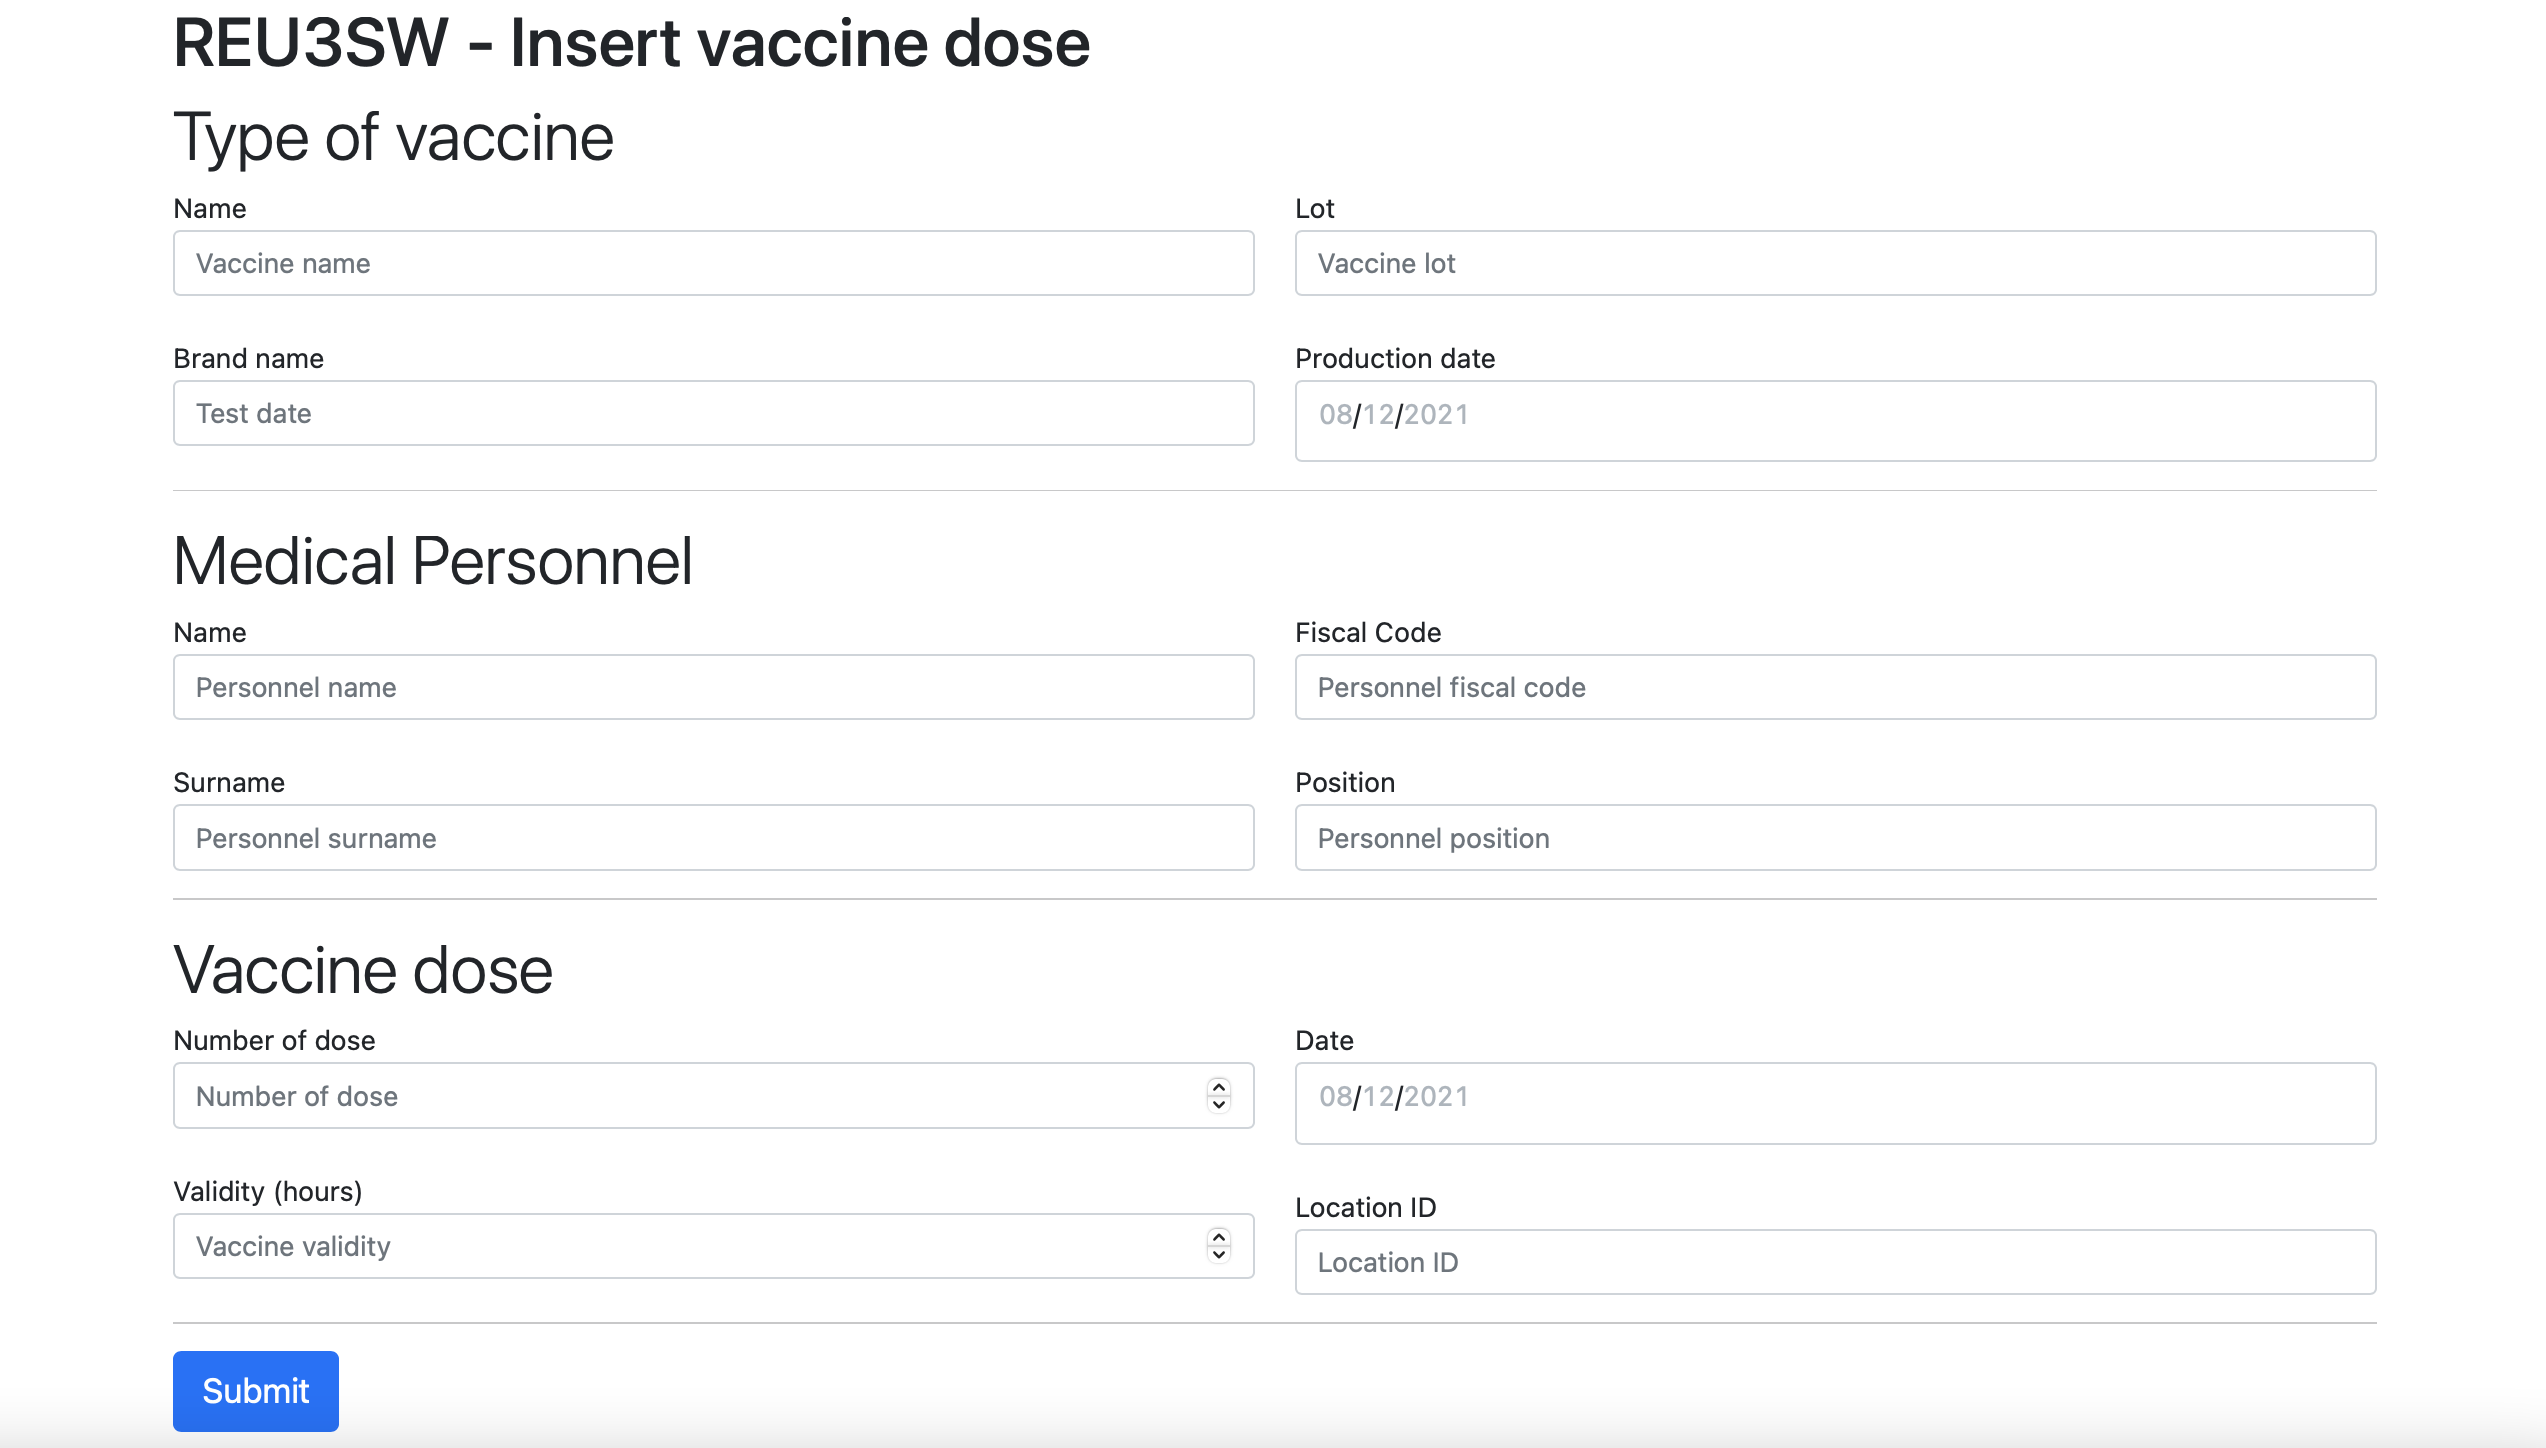
\includegraphics[scale=0.3]{screenshots/insertvaccine.png}
    \caption{Page for the insertion of a new vaccine dose to a person.}
\end{figure}
\end{document}
